%!TEX root = ../../dimensions-2016-game-book.tex


\phWorksheet{Bonus Puzzle 1}

  One of Professor W. Fayes's favorite games involved placing dominoes
  on a \(6\times6\) grid. Player \(V\) begins by placing a vertical domino,
  followed by Player \(H\) laying a domino horizontally. This process repeats
  until either \(V\) cannot lay a vertical domino without overlapping
  the dominoes on the board, or \(H\) cannot lay a horizontal domino without
  the same problem. Here's an example game that lasted \(16\) turns;
  note \(V\) would move next, but she cannot lay a vertical
  domino.

\newcommand{\phDominoVertical}[2]{
  \draw[fill=gray] ($(#1)+(0.1,0.1)$) rectangle ($(#1)+(0.9,1.9)$);
  \node at ($(#1)+(0.5,1)$) {#2};
}
\newcommand{\phDominoHorizontal}[2]{
  \draw[fill=lightgray] ($(#1)+(0.1,0.1)$) rectangle ($(#1)+(1.9,0.9)$);
  \node at ($(#1)+(1,0.5)$) {#2};
}

    \begin{center}
    \begin{tikzpicture}
      \draw[color=lightgray] (0,0) grid (6,6);
      \phDominoVertical{0,1}{1}
      \phDominoHorizontal{0,3}{2}
      \phDominoVertical{0,4}{3}
      \phDominoHorizontal{1,5}{4}
      \phDominoVertical{3,0}{5}
      \phDominoHorizontal{3,2}{6}
      \phDominoVertical{2,2}{7}
      \phDominoHorizontal{3,4}{8}
      \phDominoVertical{5,4}{9}
      \phDominoHorizontal{0,0}{10}
      \phDominoVertical{5,2}{11}
      \phDominoHorizontal{4,1}{12}
      \phDominoVertical{1,1}{13}
      \phDominoHorizontal{1,4}{14}
      \phDominoVertical{2,0}{15}
      \phDominoHorizontal{3,3}{16}
    \end{tikzpicture}
    \end{center}

    Sketch another \textit{completed} board
    below with horizontal and vertical dominoes,
    \textit{numbering the order that they were played in}. Submit your
    completed board to Game Control before the end of the game.
    Boards that are illegally constructed or
    incomplete will be disqualified.
    \textbf{The team(s) submitting a valid board using
    the least dominoes of all teams will earn this puzzle's Victory Points.}

    \begin{center}
      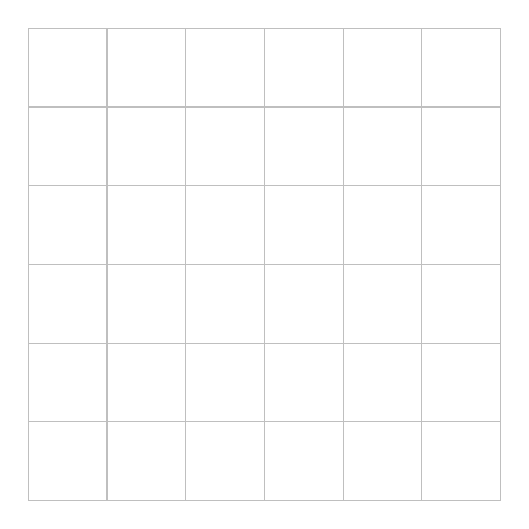
\begin{tikzpicture}
      \draw[color=lightgray] (0,0) grid (6,6);
      \end{tikzpicture}
    \end{center}

% \phWorksheet{Solutions}
%
% \begin{center}
% \phLetterBox{}{P}
% \phLetterBox{}{O}
% \phLetterBox{}{S}
% \phLetterBox{}{I}
% \phLetterBox{}{T}
% \phLetterBox{}{I}
% \phLetterBox{}{V}
% \phLetterBox{}{E}
% \end{center}
% \begin{center}
% \phLetterBox{}{R}
% \phLetterBox{}{O}
% \phLetterBox{}{T}
% \phLetterBox{}{A}
% \phLetterBox{}{T}
% \phLetterBox{}{I}
% \phLetterBox{}{O}
% \phLetterBox{}{N}
% \end{center}
%
% (the unused letters spell DECIPHER THE MOTTO)